\documentclass[12pt]{exam}
\usepackage[utf8]{inputenc}
\usepackage[margin=1in]{geometry}
\usepackage{amsmath,amssymb}
\usepackage{multicol}
\usepackage[english]{babel}
\usepackage{graphicx}
\usepackage{tikz}
\usepackage{float}
\usepackage{etoolbox} % Required for \ifblank
\usepackage{xcolor} % Required for comments or highlighting
\usepackage{tabularx}
\usepackage{setspace} % Required for setting line spacing


\newcommand{\class}{Automotive Technology}
\newcommand{\term}{DE-43 MTS}
\newcommand{\examnum}{Final Exam}
\newcommand{\examdate}{May 23, 2024}
\newcommand{\timelimit}{3 hours}
\newcommand{\classcode}{ME-443}
\newcommand{\timing}{0930-1230 hrs}
\newcommand{\maxmarks}{100}
\newcommand{\Instructor}{Usman Asad}

\pagestyle{head}
\firstpageheader{\textbf{CMS ID} & \makebox[1.8in]{\hrulefill}}{}{\textbf{Name} & \makebox[1.8in]{\hrulefill}}
\runningheader{}{Page \thepage\ of \numpages}{}
\runningheadrule


% Top Stuff
\begin{document}
	\begin{tikzpicture}[remember picture,overlay]
    	\node[xshift=25 mm,yshift=-30 mm,anchor=north west] at (current page.north west){%
    		\includegraphics[width=24mm]{NUST}};
    	\end{tikzpicture}
    	
    		\begin{tikzpicture}[remember picture,overlay]
    	\node[xshift=-25 mm,yshift=-30 mm,anchor=north east] at (current page.north east){%
    		\includegraphics[width=24mm]{CEME}};
	\end{tikzpicture}
	
	
\begin{center}
	\textbf{National University of Sciences and Technology}\\
	\textbf{College of E\&ME (Department of Mechatronics)}\\
	\textbf{\examnum (\term)}\\
\end{center}

	
	% Exam Details
	\noindent
	\\
	\begin{tabular*}{\textwidth}{l @{\extracolsep{\fill}} r @{\extracolsep{6pt}} l}
		\textbf{Subject Code: }\classcode &&\textbf{Subject: }\class \\
		\textbf{Date: }\examdate && \textbf{Timing: }\timing\\
		\textbf{Time Limit: }\timelimit && \textbf{Max Marks: }\maxmarks\\
		\textbf{Instructor: }\Instructor
	\end{tabular*}\\
	\rule[2ex]{\textwidth}{1pt}
	\textbf{Instructions:}\\This exam contains \numpages\ pages. Please solve the exam on the question paper. \textbf{You do not need an answer sheet}. You may request a continuation sheet if needed. \\ \\
	\rule[2ex]{\textwidth}{1pt}
    
\noindent{Mark the answers for \textbf{True/False} Questions here} \\
\begin{tabular*}{\textwidth}{@{\extracolsep{\fill}}p{0.2\textwidth}p{0.2\textwidth}p{0.2\textwidth}p{0.2\textwidth}}
% \hline
1. $\textcircled{T} \textcircled{F}$ & 6. $\textcircled{T} \textcircled{F}$ & 11. $\textcircled{T} \textcircled{F}$ & 15. $\textcircled{T} \textcircled{F}$ \\
% \hline
2. $\textcircled{T} \textcircled{F}$ & 7. $\textcircled{T} \textcircled{F}$ & 12. $\textcircled{T} \textcircled{F}$ & 16. $\textcircled{T} \textcircled{F}$ \\
% \hline
3. $\textcircled{T} \textcircled{F}$ & 8. $\textcircled{T} \textcircled{F}$ & 13. $\textcircled{T} \textcircled{F}$ & 17. $\textcircled{T} \textcircled{F}$ \\
% \hline
4. $\textcircled{T} \textcircled{F}$ & 9. $\textcircled{T} \textcircled{F}$ & 14. $\textcircled{T} \textcircled{F}$ & 18. $\textcircled{T} \textcircled{F}$ \\
% \hline
5. $\textcircled{T} \textcircled{F}$ & 10. $\textcircled{T} \textcircled{F}$ &  &  \\
% \hline
\end{tabular*}

\vspace{1cm}

\noindent{Mark the answers for \textbf{Multiple Choice Questions} here} \\
\begin{tabular*}{\textwidth}{@{\extracolsep{\fill}}p{0.24\textwidth}p{0.24\textwidth}p{0.24\textwidth}p{0.24\textwidth}}
% \hline
1. $\textcircled{a} \textcircled{b} \textcircled{c} \textcircled{d}$ & 7. $\textcircled{a} \textcircled{b} \textcircled{c} \textcircled{d}$ & 13. $\textcircled{a} \textcircled{b} \textcircled{c} \textcircled{d}$ & 18. $\textcircled{a} \textcircled{b} \textcircled{c} \textcircled{d}$ \\
% \hline
2. $\textcircled{a} \textcircled{b} \textcircled{c} \textcircled{d}$ & 8. $\textcircled{a} \textcircled{b} \textcircled{c} \textcircled{d}$ & 14. $\textcircled{a} \textcircled{b} \textcircled{c} \textcircled{d}$ & 19. $\textcircled{a} \textcircled{b} \textcircled{c} \textcircled{d}$ \\
% \hline
3. $\textcircled{a} \textcircled{b} \textcircled{c} \textcircled{d}$ & 9. $\textcircled{a} \textcircled{b} \textcircled{c} \textcircled{d}$ & 15. $\textcircled{a} \textcircled{b} \textcircled{c} \textcircled{d}$ & 20. $\textcircled{a} \textcircled{b} \textcircled{c} \textcircled{d}$ \\
% \hline
4. $\textcircled{a} \textcircled{b} \textcircled{c} \textcircled{d}$ & 10. $\textcircled{a} \textcircled{b} \textcircled{c} \textcircled{d}$ & 16. $\textcircled{a} \textcircled{b} \textcircled{c} \textcircled{d}$ & 21. $\textcircled{a} \textcircled{b} \textcircled{c} \textcircled{d}$ \\
% \hline
5. $\textcircled{a} \textcircled{b} \textcircled{c} \textcircled{d}$ & 11. $\textcircled{a} \textcircled{b} \textcircled{c} \textcircled{d}$ & 17. $\textcircled{a} \textcircled{b} \textcircled{c} \textcircled{d}$ & 22. $\textcircled{a} \textcircled{b} \textcircled{c} \textcircled{d}$ \\
% \hline
6. $\textcircled{a} \textcircled{b} \textcircled{c} \textcircled{d}$ & 12. $\textcircled{a} \textcircled{b} \textcircled{c} \textcircled{d}$ & &  \\
% \hline
\end{tabular*}




        \begin{center}

            \textbf{Fill in the blanks} in the provided space
        \end{center}
        \begin{questions}
        
		
		% \renewcommand{\baselinestretch}{3}
		
        \question A \textbf{METERING} valve is used on front-disc, rear-drum brake systems to delay front brake application until rear brakes engage. % Answer: metering (Page 1046)
        \question In the context of steering, EPAS stands for electric \textbf{POWER ASSISTED STEERING}
        \question In the context of braking, EBCM stands for\textbf{ Electronic Brake Control Module}
        \question In a leaf spring suspension, \textbf{Rebound Clips} help prevent the leaves from separating whenever the leaf spring is rebounding from hitting bump or rise in the roadway.
        \question In a leaf spring suspension, the leafs are held together by a \textbf{Center Bolt / Centering Pin}
        \question The two most common types of front suspension used in passenger cars are the \textbf{MacPherson Strut} and \textbf{SLA / Double Wishbone} suspension.
        \question A combination valve in a braking system contains a Pressure-Differential Switch, a \textbf{Metering Valve} and a \textbf{Proportioning Valve}.
        \question A \textbf{variable steering ratio }is obtained by using a rack-and-pinion gear set that has a different tooth pitch in the center than it has on the outside.
        \end{questions}
        \setcounter{question}{0}




	\begin{questions}
		% True False
        \addpoints
        %\pointsinleftmargin
        %\boxedpoints
		% \question[18]
        \begin{center}            
    \textbf{True/False:} Mark these statements as True or false on the table in the front page.
       \end{center}
		% % \begin{enumerate}		     
            \question Multi-grade engine oils (e.g., 10W-30) have a viscosity that changes significantly with temperature, becoming much thicker when hot. % False (General lubrication knowledge - designed to be more stable, the 'W' indicates winter viscosity, second number is at operating temp)
            \question Brake fluid level in the master cylinder reservoir typically rises as brake pads wear.
            \question Drum brakes are generally more resistant to heat-induced fade than disc brakes. % False (Page 1115, Chapter 101 - Disc brakes have better fade resistance)
            \question The radiator cap is designed to increase the boiling point of coolant by pressurizing the cooling system. % True
            % \question Oil viscosity decreases as engine temperature increases. % True
            \question The transfer case in a four-wheel drive vehicle is responsible for sending power to both the front and rear axles. % True
            \question A solid axle suspension provides better handling and comfort than an independent suspension system. % False
            \question Disc brakes are more prone to fading under heavy use compared to drum brakes. % False
            \question In a diagonal split braking system, if one circuit fails, the vehicle will lose all braking power. % False (Page 1036, Chapter 94 - remaining circuit can still stop the vehicle)
			\question A strut is a sturdy shock absorber that is also a structural component of the suspension.						
			\question One end of a torsion bar is attached to the lower control arm of a front suspension and the other to the upper control arm.
			\question Most master cylinder reservoirs for brake fluid are see-through, to allow brake fluid level to be checked without remove the top.
			\question Standard shock absorbers support the weight of the vehicle
			\question For a constant steering ratio, lower steering effort is required at the edge of range of motion of the wheel.
            \question Antilock braking systems (ABS) are designed to release the brakes when slip is at 100\%.
            \question Parallelogram steering units do not require a Rack-and-pinion %True.
            \question A high steering gear ratio, such as 22:1, means that the steering wheel is harder to turn than a steering wheel with a lower ratio like 14:1. 
            \question The short-long-arm suspension uses a longer upper control arm and a shorter lower control arm.
            \question The vacuum power booster is a component that reduces the driver's effort but does not reduce stopping distance.           
		% \end{enumerate}
		
		
		
		
			% changing choice items style locally
		
			% %
        \end{questions}
			\begin{center} 

            \textbf{MCQs: }Multiple Choice Questions. Mark the answers on the front page. 
            \end{center}

     	\renewcommand*\thechoice{\alph{choice}} 
			\renewcommand*\choicelabel{\thechoice)}
        \setcounter{question}{0}
        \begin{questions}           

                \question Which steering component is responsible for converting the rotary motion of the steering wheel into linear motion to move the tie rods in a rack-and-pinion system? \\ % (Page 1367, Chapter 116)
                \begin{oneparchoices}
                    \choice Pitman arm
                    \choice Sector gear
                    \choice Pinion gear % Answer: Pinion gear
                    \choice Ball nut
                \end{oneparchoices}
 
                \question The split point in a proportioning valve refers to the: \\ % (Page 1044, Chapter 95)
				\begin{oneparchoices}					
					\choice Pressure at which the valve begins to reduce pressure to the rear brakes. \\% Answer: Pressure at which the valve begins to reduce pressure to the rear brakes.
					\choice Point where the brake pedal linkage splits to two master cylinder circuits.\\
					\choice Temperature at which brake fluid begins to boil. \\
					\choice Difference in pressure that activates the brake warning light.
				\end{oneparchoices}
                
				    \question Which of the following components helps regulate engine temperature by opening and closing based on coolant temperature? \\
                    \begin{oneparchoices}
                        \choice Radiator
                        \choice Water pump
                        \choice Thermostat % Correct
                        \choice Expansion tank
                    \end{oneparchoices}
                    
				\question In coolant tests, the density of the coolant is determined by \\
				\begin{oneparchoices}					
						\choice Hydrometer
						\choice Refractometer \\
						\choice pH testing
						\choice Galvanic activity and electrolysis testing
				\end{oneparchoices}
							
				\question What is the purpose of strut rods in a vehicle’s suspension system? \\
				 \begin{oneparchoices} 
					\choice To provide forward/backward support to the control arms \\
					\choice To prevent excessive body roll while cornering \\
					\choice To add stability while driving over rough road surfaces \\
					\choice To increase the effective force of the stabilizer bar
				\end{oneparchoices}
                \question The primary purpose of a vacuum valve in a radiator pressure cap is to: \\ % (Cooling System Lec, Slide 15)
                \begin{oneparchoices}
                    \choice Release excess pressure from the cooling system.\\
                    \choice Allow coolant to flow back into the radiator as the system cools and contracts. \\ % Answer: Allow coolant to flow back into the radiator as the system cools and contracts.
                    \choice Prevent coolant from freezing. \\
                    \choice Increase the boiling point of the coolant.
                \end{oneparchoices}
                
                \question Which of the following describes a rich mixture in an engine? \\ % (Air/Fuel Induction Lec, Slide 6)
                \begin{oneparchoices}
                    \choice Too much air for the amount of fuel. \\
                    \choice The ideal air-fuel ratio for complete combustion. \\
                    \choice Too much fuel for the amount of air. \\ % Answer: Too much fuel for the amount of air.
                    \choice Not enough fuel for the air in the cylinders.
                \end{oneparchoices}

                
                \question The lowest temperature at which oil will pour is called its: \\ % (Lubrication System Lec, Slide 14)
                \begin{oneparchoices}
                    \choice Flash point
                    \choice Viscosity index
                    \choice Pour point  % Answer: Pour point
                    \choice SAE grade
                \end{oneparchoices}
                \question In a part-time 4WD system, driving on dry pavement in 4WD mode can cause: \\ % (General 4WD knowledge)
				 \begin{oneparchoices} 
					\choice Improved fuel economy.
					\choice Drivetrain binding or "wind-up". \\ % Answer: Drivetrain binding or "wind-up".
					\choice Smoother cornering.
					\choice Reduced tire wear.
				\end{oneparchoices}
                
                \question The MAF sensor in a modern fuel injection system measures: \\ % (General air/fuel system knowledge)
				\begin{oneparchoices} 
					\choice Manifold Absolute Pressure
					\choice Mass Air Flow \\ % Answer: Mass Air Flow
					\choice Throttle Position
					\choice Engine Coolant Temperature
				\end{oneparchoices}

                
			    \question Which suspension component is responsible for absorbing shock and controlling spring motion? \\
                \begin{oneparchoices}
                    \choice Coil spring
                    \choice Stabilizer bar
                    \choice Shock absorber % Correct
                    \choice Control arm
                \end{oneparchoices}
				\question What is the purpose of shackles in a leaf spring suspension system? \\
				\begin{oneparchoices} 
					\choice To allow for rearward movement of the spring as it hits a bump \\ 
					\choice To prevent the leaves from separating during rebound \\
					\choice To isolate road noise from traveling into the passenger compartment \\
					\choice To attach the leaf spring to the frame
				 \end{oneparchoices}
			 
				\question In a Master Cylinder, the Replenishing Port is also called the  \\
				\begin{oneparchoices}					
					\choice Compensating Port
					\choice Vent Port
					\choice Inlet Port
					\choice Pushrod Port
				\end{oneparchoices}
			
				\question What is the purpose of the filter bypass valve in an oil filter? \\
				\begin{oneparchoices} 
					\choice To remove small particles from oil \\
					\choice To prevent oil from draining out of the filter \\
					\choice To open if too much pressure is formed in the filter \\
					\choice To protect the engine from oil starvation 
				\end{oneparchoices}
			
				\question If there is a leak in the braking system, it will cause unequal pressure going to the front and rear. This is detected by the  \\
				\begin{oneparchoices}					
					\choice Metering Valve
					\choice Proportioning Valve \\
					\choice Master Cylinder
					\choice Pressure-Differential Switch					
				\end{oneparchoices}
				
				\question What does the steering gear ratio represent? \\
				\begin{oneparchoices} 
					\choice Steering wheel rotation to move front wheels 1 degree \\ 
                    \choice Steering wheel revolutions from full left to full right \\
					\choice Front wheel rotation range \\
					\choice Force required to turn the steering wheel 
				\end{oneparchoices}
				
				\question A pitman shaft is also known as a \\
				\begin{oneparchoices} 
					\choice Sector Shaft
					\choice Worm Shaft
					\choice Counter Shaft
					\choice Main shaft
				\end{oneparchoices}
				
				\question What is the purpose of a metering valve in a vehicle’s braking system? \\
				\begin{oneparchoices} 
					\choice To prevent the full operation of the disc brakes until sufficient pressure is sent to the rear drum brakes \\
					\choice To allow the front and rear brakes to apply at the same time for even stopping \\
					\choice To prevent front brake locking under light pedal pressures on icy surfaces \\
					\choice All of the above 
				\end{oneparchoices}
			
				
			
				\question What is the main characteristic of unit-body construction in vehicles? \\
				\begin{oneparchoices} 
					\choice The body is composed of many individual stamped-steel panels welded together \\
					\choice The body is made of a single piece of steel \\
					\choice The body is attached to a separate frame \\
					\choice The body is made of lightweight materials such as aluminum or carbon fiber 
				\end{oneparchoices}

                 \question The weight supported by the suspension is called \_\_\_\_\_\_\_\_ weight. \\
                \begin{oneparchoices} 
                    \choice sprung
                    \choice unsprung
                    \choice total
                    \choice gross
                \end{oneparchoices}

                \question  Which of the following best describes wind-up? \\
                \begin{oneparchoices}
                    \choice Excessive tire wear due to aggressive off-road driving.\\
                    \choice The twisting of drivetrain components (such as driveshafts) when the front and rear wheels rotate at different speeds.\\
                    \choice A sudden loss of traction during acceleration.\\
                    \choice The tendency of 4WD vehicles to roll over during sharp turns.
                \end{oneparchoices}
                                
                \question The \_\_\_\_\_\_\_\_ bar is used to prevent excessive body roll while cornering and to add stability while driving over rough road surfaces. \\
                \begin{oneparchoices} 
                    \choice stabilizer
                    \choice torsion
                    \choice sway
                    \choice control
                \end{oneparchoices}


                
		
			
		


            
        \end{questions}
        \setcounter{question}{0}
        \begin{center}

            \textbf{Short Questions:} Provide brief answers to the following within the space provided. Sample answers by Gemini:
        \end{center}
        \begin{questions}
		

    
        \question[6] Summarize some useful details about any two lubrication additives
        \begin{itemize}
            \item \textbf{Viscosity Index Improvers:} Reduce the rate at which a lubricant's viscosity decreases as temperature increases, ensuring consistent lubrication across a wider temperature range.
            \item \textbf{Antioxidants:} Prevent or slow down the oxidation of the lubricant, which can lead to sludge and varnish formation, extending the oil's lifespan.
            \item \textbf{Anti-wear Agents:} Form a protective film on metal surfaces under high load and temperature conditions, reducing direct contact and wear.
            \item \textbf{Detergents/Dispersants:} Keep engine parts clean by neutralizing acids and preventing the formation of deposits like sludge and varnish.
        \end{itemize}
        \question[4] CLO1/PLO2: Why is an inert gas used in a gas-charged shock absorber \\
        An inert gas, typically nitrogen, is used to prevent cavitation (formation of vapor bubbles in the hydraulic fluid). The gas maintains positive pressure on the fluid, suppressing bubble formation under rapid or repeated shock loads, ensuring consistent damping performance.
                
        \question[4] CLO1/PLO2: Why is a planetary gear set used in a column-assisted electric power steering system? \\
        If the electric motor (connected to a worm gear acting as the sun gear) fails, the steering mechanism will not become locked. The planetary gear set still allows for manual steering with the inherent gear reduction, providing a crucial safety feature.
            

  
		

			
	
        
            \question[36] CLO2/PLO3: For the diagrams on the next page, write down the number corresponding to each of these components. Note that you don't have to name all of the numbered parts. For example, number 39 is the Clutch Disk, so just write 39 in the column after Clutch Disk, as shown.
    \end{questions}
        \begin{center}
\begingroup % Start a new scope for spacing changes
% \setstretch{1.5} % Double the line spacing within this group
\doublespacing
\begin{tabular}{| m{13em} | m{2cm}| m{13em} | m{2cm}|}
\hline
\textbf{Component} & \textbf{Number} & \textbf{Component} & \textbf{Number} \\
\hline
Clutch Disk & 39 & Stabilizer Bar & 47 \\ \hline
Axle Shaft & 8 or 5& Diaphgram Spring & 36 or 37\\ \hline
Flywheel & 41 & Pitman Arm & 22 \\ \hline
Clutch Hub & 45 & Throwout Bearing & No number \\ \hline
Steering Knuckle & 21 & Worm Gear & 26 \\ \hline
Spindle & 19 & Drive Shaft & 2\\ \hline
Guide Pins & 10 & Strut Rod & 17 \\ \hline
Ring Gear & 1 & Upper Control Arm & 20 \\ \hline
Synchronizer Sleeve & 44 & Pinion Gear & 3\\ \hline
Shock Absorber &16 & Side Gear &6 \\ \hline
Spider Gear &7 & Wheel Cylinder & 31 \\ \hline
Return Spring & 28 or 30 & Anchor & 29\\ \hline
Brake Pad &13 & Key Springs & 46 \\ \hline
Starwheel & 34 & Pressure Plate & 38\\ \hline
Steering Shaft & 23 & Rotor & 11 or 12\\ \hline
Synchronizer Ring  & 42 & Ball Nut Rak & 24 \\ \hline
Sector Gear & 27 & Speed Gear & 43\\ \hline
Coil Spring & 15 & Holddown & 32\\ \hline
Recirculating Ball Bearings & 25 & Caliper Assembly &9 \\ \hline

\hline
\end{tabular}
\endgroup % End the scope of spacing changes
\end{center}
% \end{questions}

%\gradetable[h][questions]
%	\begin{tabular}{|c|c|c|c|c|c|c|c|c|c|c|c|c|c|} 
%		\hline Q1 & Q2 & Q3 & Q4a & Q4b & Q4c & Q4d & Q4e & Q4f & Q4g & Q4h & Q4i & Q4j & Total \\ 
%		\hline & & & & & & & & & & & & & \\
%		& & & & & & & & & & & & & \\
%		\hline 
%	\end{tabular}
\clearpage % Or \newpage
 % Insert a non-visible element
\begin{figure}[p]
    \centering
    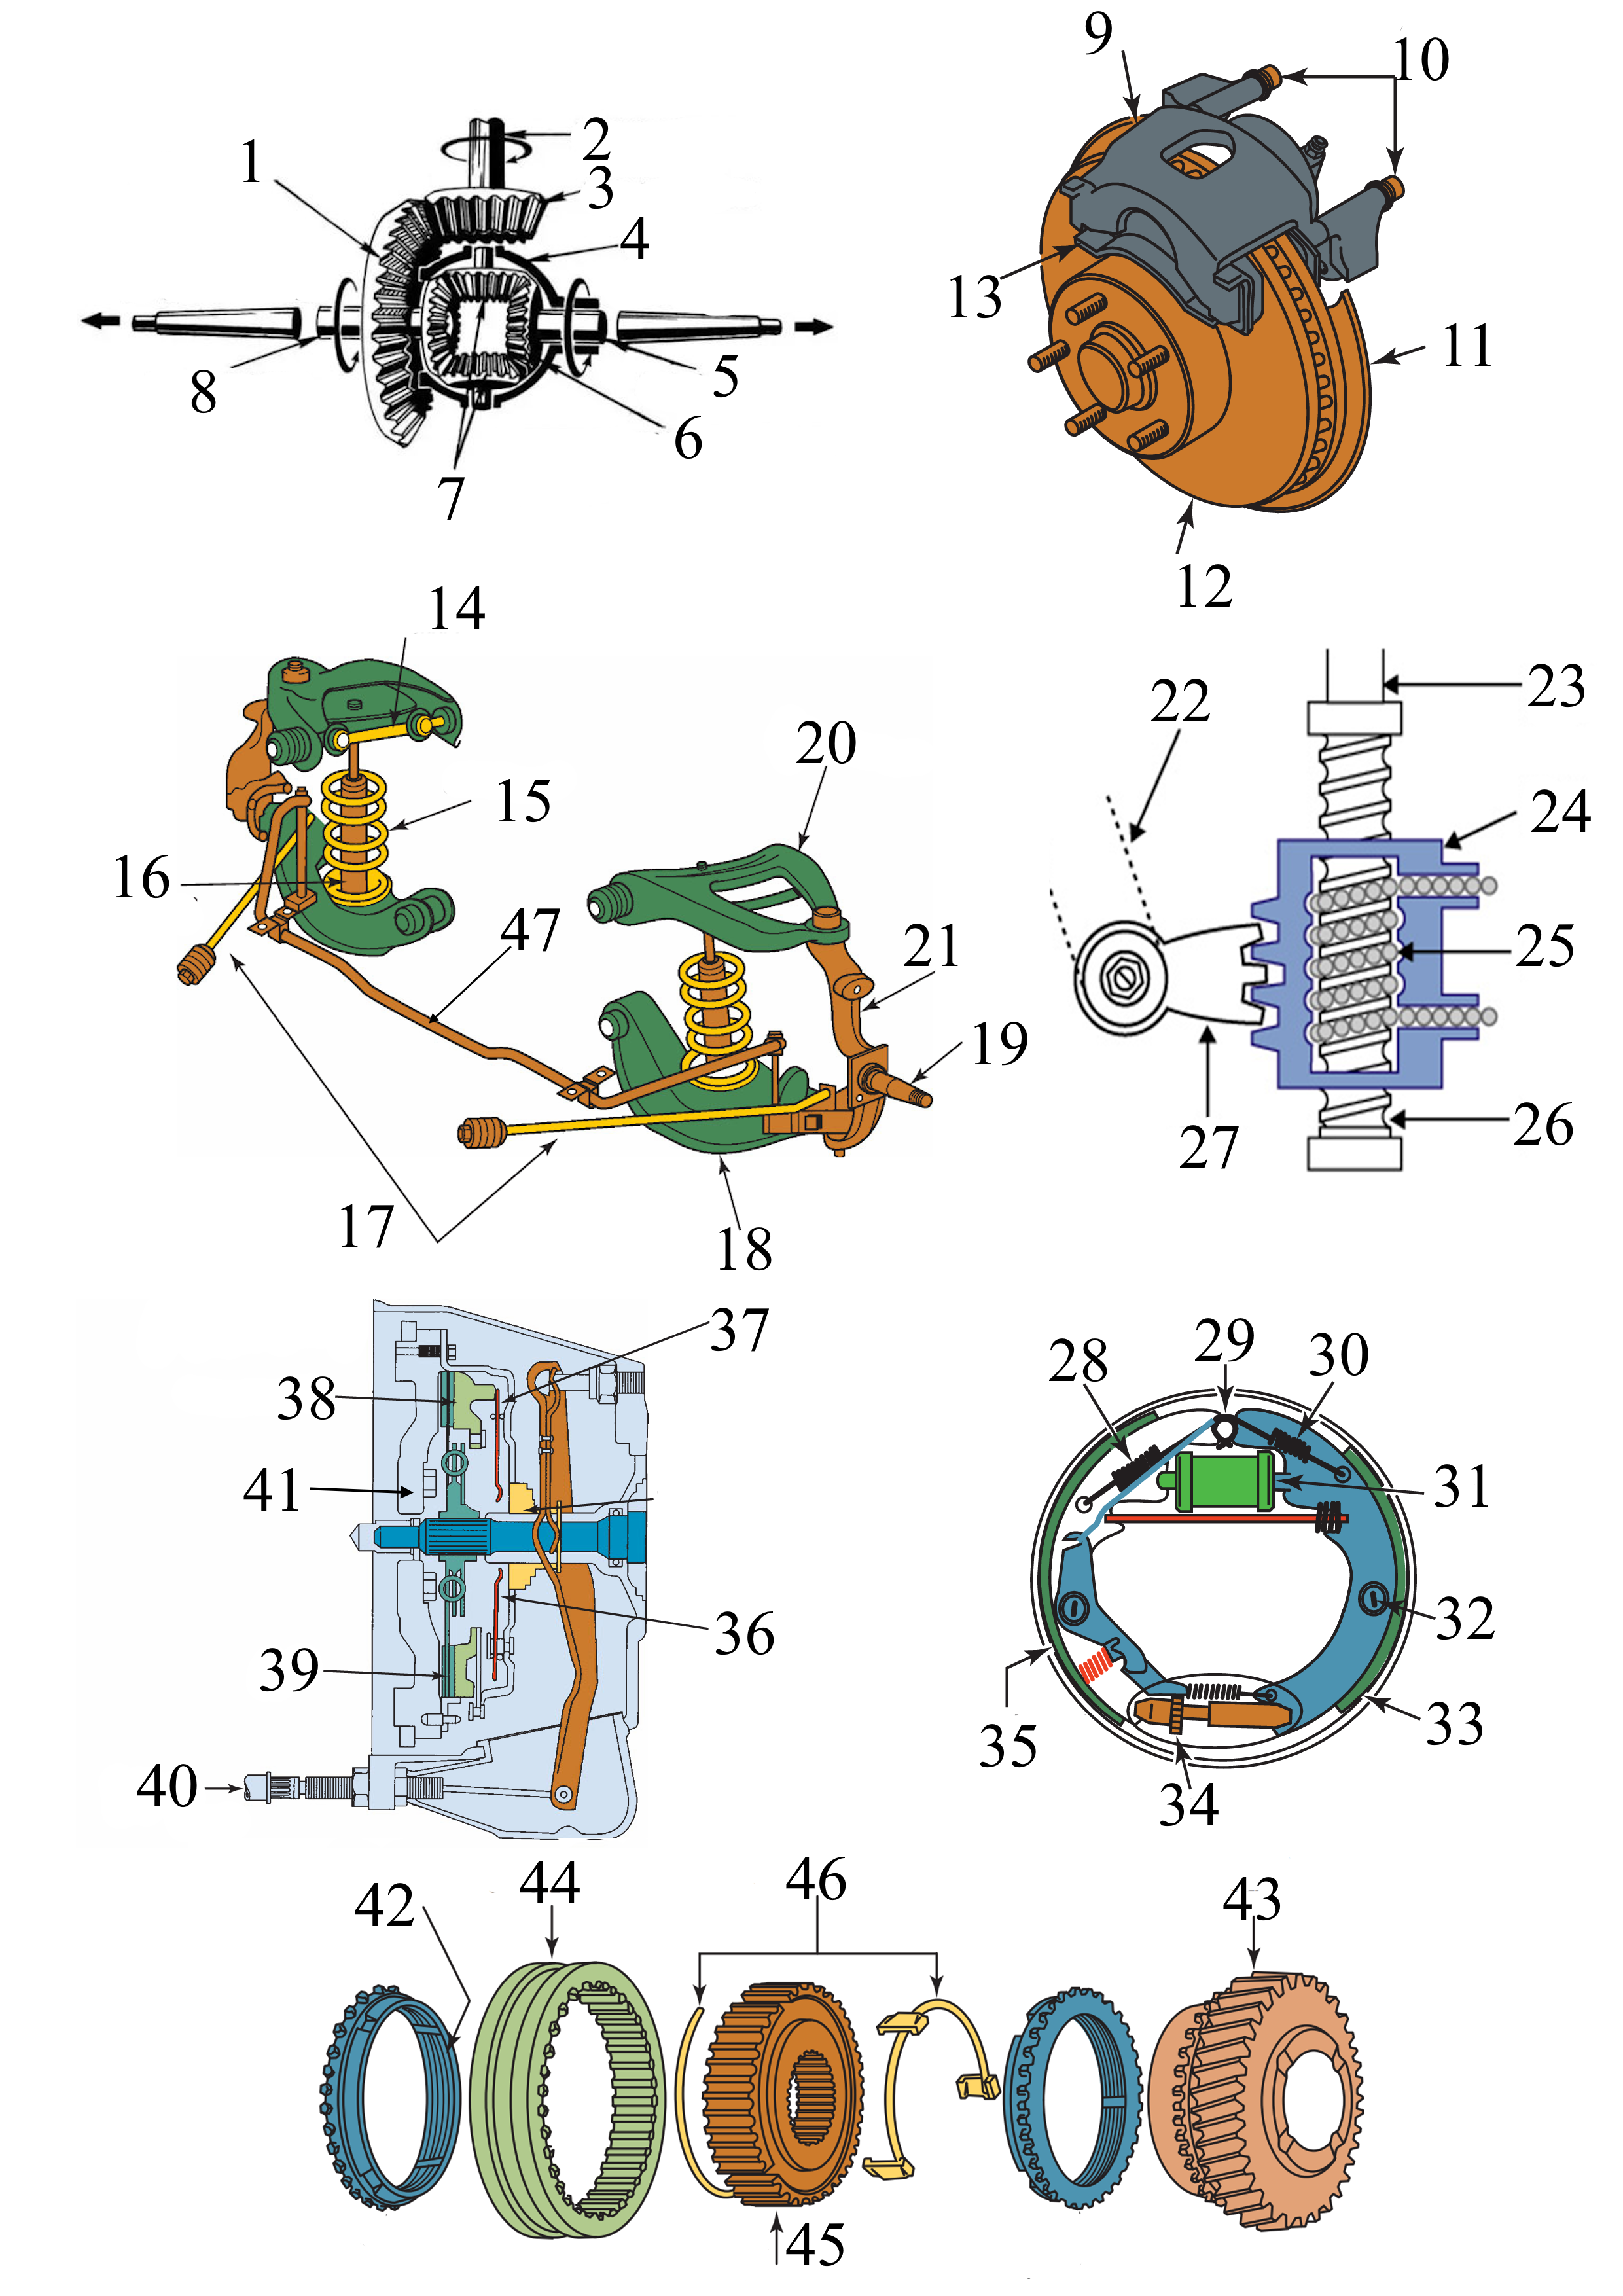
\includegraphics[width=1\linewidth]{Labels.png}
\end{figure}
\clearpage % Force a new page after the nu

\end{document}
